\addcontentsline{toc}{part}{Conclusion et Bilan}
\newgeometry{height=10in}.

\chapter*{Conclusion et Bilan}
\setcounter{section}{0}


\section*{Bilan du chef de projet}

\subsection*{Bilan global}
Le projet s'est dans l'emsemble bien déroulé. Le principal problème de ce projet a été de constamment devoir recommencer les différents diagrammes jusqu'à ce qu'ils soient corrects. De plus, il existe peu d'outils qui soient réellement pratiques pour la réalisation de ces projets, surtout en ce qui concerne les IHM.

\subsection*{Outils utilisés}
Dans le but d'harmoniser l'ensemble du rendu, nous avons choisi d'utiliser \textbf{PlantUML} pour réaliser l'ensemble des diagrammes. La possibilité d'utiliser des variables pour les différents diagrammes nous a permis de détecter et d'éviter les redondances au niveau des services métiers. Le principal problème avec cet outil est qu'il est difficile de s'éloigner de l'UML standard (exemple : impossible de créer plusieurs "endPoints" dans les diagrammes d'activités).\\

Les IHM ont été réalisées à l'aide de \textbf{Balsamiq}, qui est malheureusement un des seuls outils qui permettent d'aller assez rapidement. Mais l'export pdf final est très décevant au niveau qualité. \\

L'ensemble du suivi du projet a été effectué sur \textbf{Redmine}. Nous n'avons pas trop utilisé l'affectatioin des tâches à des personnes car il était nécessaire que plusieurs personnes relisent les différents diagrammes pour s'assurer de leur cohérence avec le reste. Ainsi, les tâches étaient données oralement, et les différents membres de l'équipe devaient néanmoins indiquer le temps passé sur les différentes tâches sur le \textbf{Redmiine}.

\subsection*{Bilan sur le temps de travail}
  \begin{figure}[H]
    \begin{tikzpicture}
      \begin{axis}[
        mbarplot,
        ylabel=Temps (Heures),
        axis y line=left,
        axis x line=bottom,
        xmin=0, xmax=5,
        ymin=0, ymax=40,
        xtick={1,2,3,4},
        xticklabels={Conception\\ d’ensemble,Conception\\ fonctionnelle\\ détaillée,Conception\\ applicative\\ détaillée,Architecture\\ technique},%<--Here
        xlabel style={yshift=-1cm},
        x tick label style={
            rotate=62,
            anchor=east,
            font=\footnotesize,
            align=right
        },
        width=\textwidth,
        height=7cm,
      ]

      \addplot plot coordinates {(1, 20) (2, 25) (3, 22.4) (4, 12.4)};
      \addplot plot coordinates {(1, 18) (2, 24) (3, 23.5) (4, 13.2)};

      \legend{Temps estimé, Temps passé}

      \end{axis}
    \end{tikzpicture}
  \end{figure}
  
Le lecteur peut trouver ci-dessus un graphique indiquant le temps mis par l'équipe sur chaque tâche.
On constate un dépassement du temps estimé pour la réalisation du projet, en particulier du au fait qu'il a fallu recommencer plusieurs fois les diagrammes à cause de certains aspects métiers peu clairs et/ou mal compris (ex : contact prévu/affecté, plusieurs rendez-vous par contact, organisation de la proposition commerciale, etc...)


\todo[inline]{insérer un graphique des temps}
La durée totale a été de \todo[inline]{insérer le temps} heures. Ceci correspond à environ ... heures par membres de l'équipe du projet.\\

Les dépassements de temps ont été du au fait qu'il fallait une compréhension de la globalité du projet par l'ensemble des membres de l'équipe, car il comprenait de nombreuses petites substilités. De ce fait, les travaux de relectures des travaux et de compréhension des travaux des autres personnes du projet ont entrainé des dépassements de temps sur de nombreuses tâches. Ceci a néanmoins permi d'assurer un travail cohérent dans la globalité, ainsi qu'une meilleur compréhension des problèmes.\\

Le challenge de ce type de projet a été d'assuré une bonne communication globale entre les membres du projet. Nous avons utilisé l'outil collaboratif \textbf{Slack} pour ceci ainsi q'un répertoire \textbf{Git} pour échanger le code \textbf{PlantUML}. Malheuresement, les fichiers d'IHM étaient difficilement versionnables, et ceci nous empechaient à travailler à plusieurs dessus du fait de la difficulté à fusionner le travail de plusieurs membres.

\subsection*{Analyse du temps passé par partie}

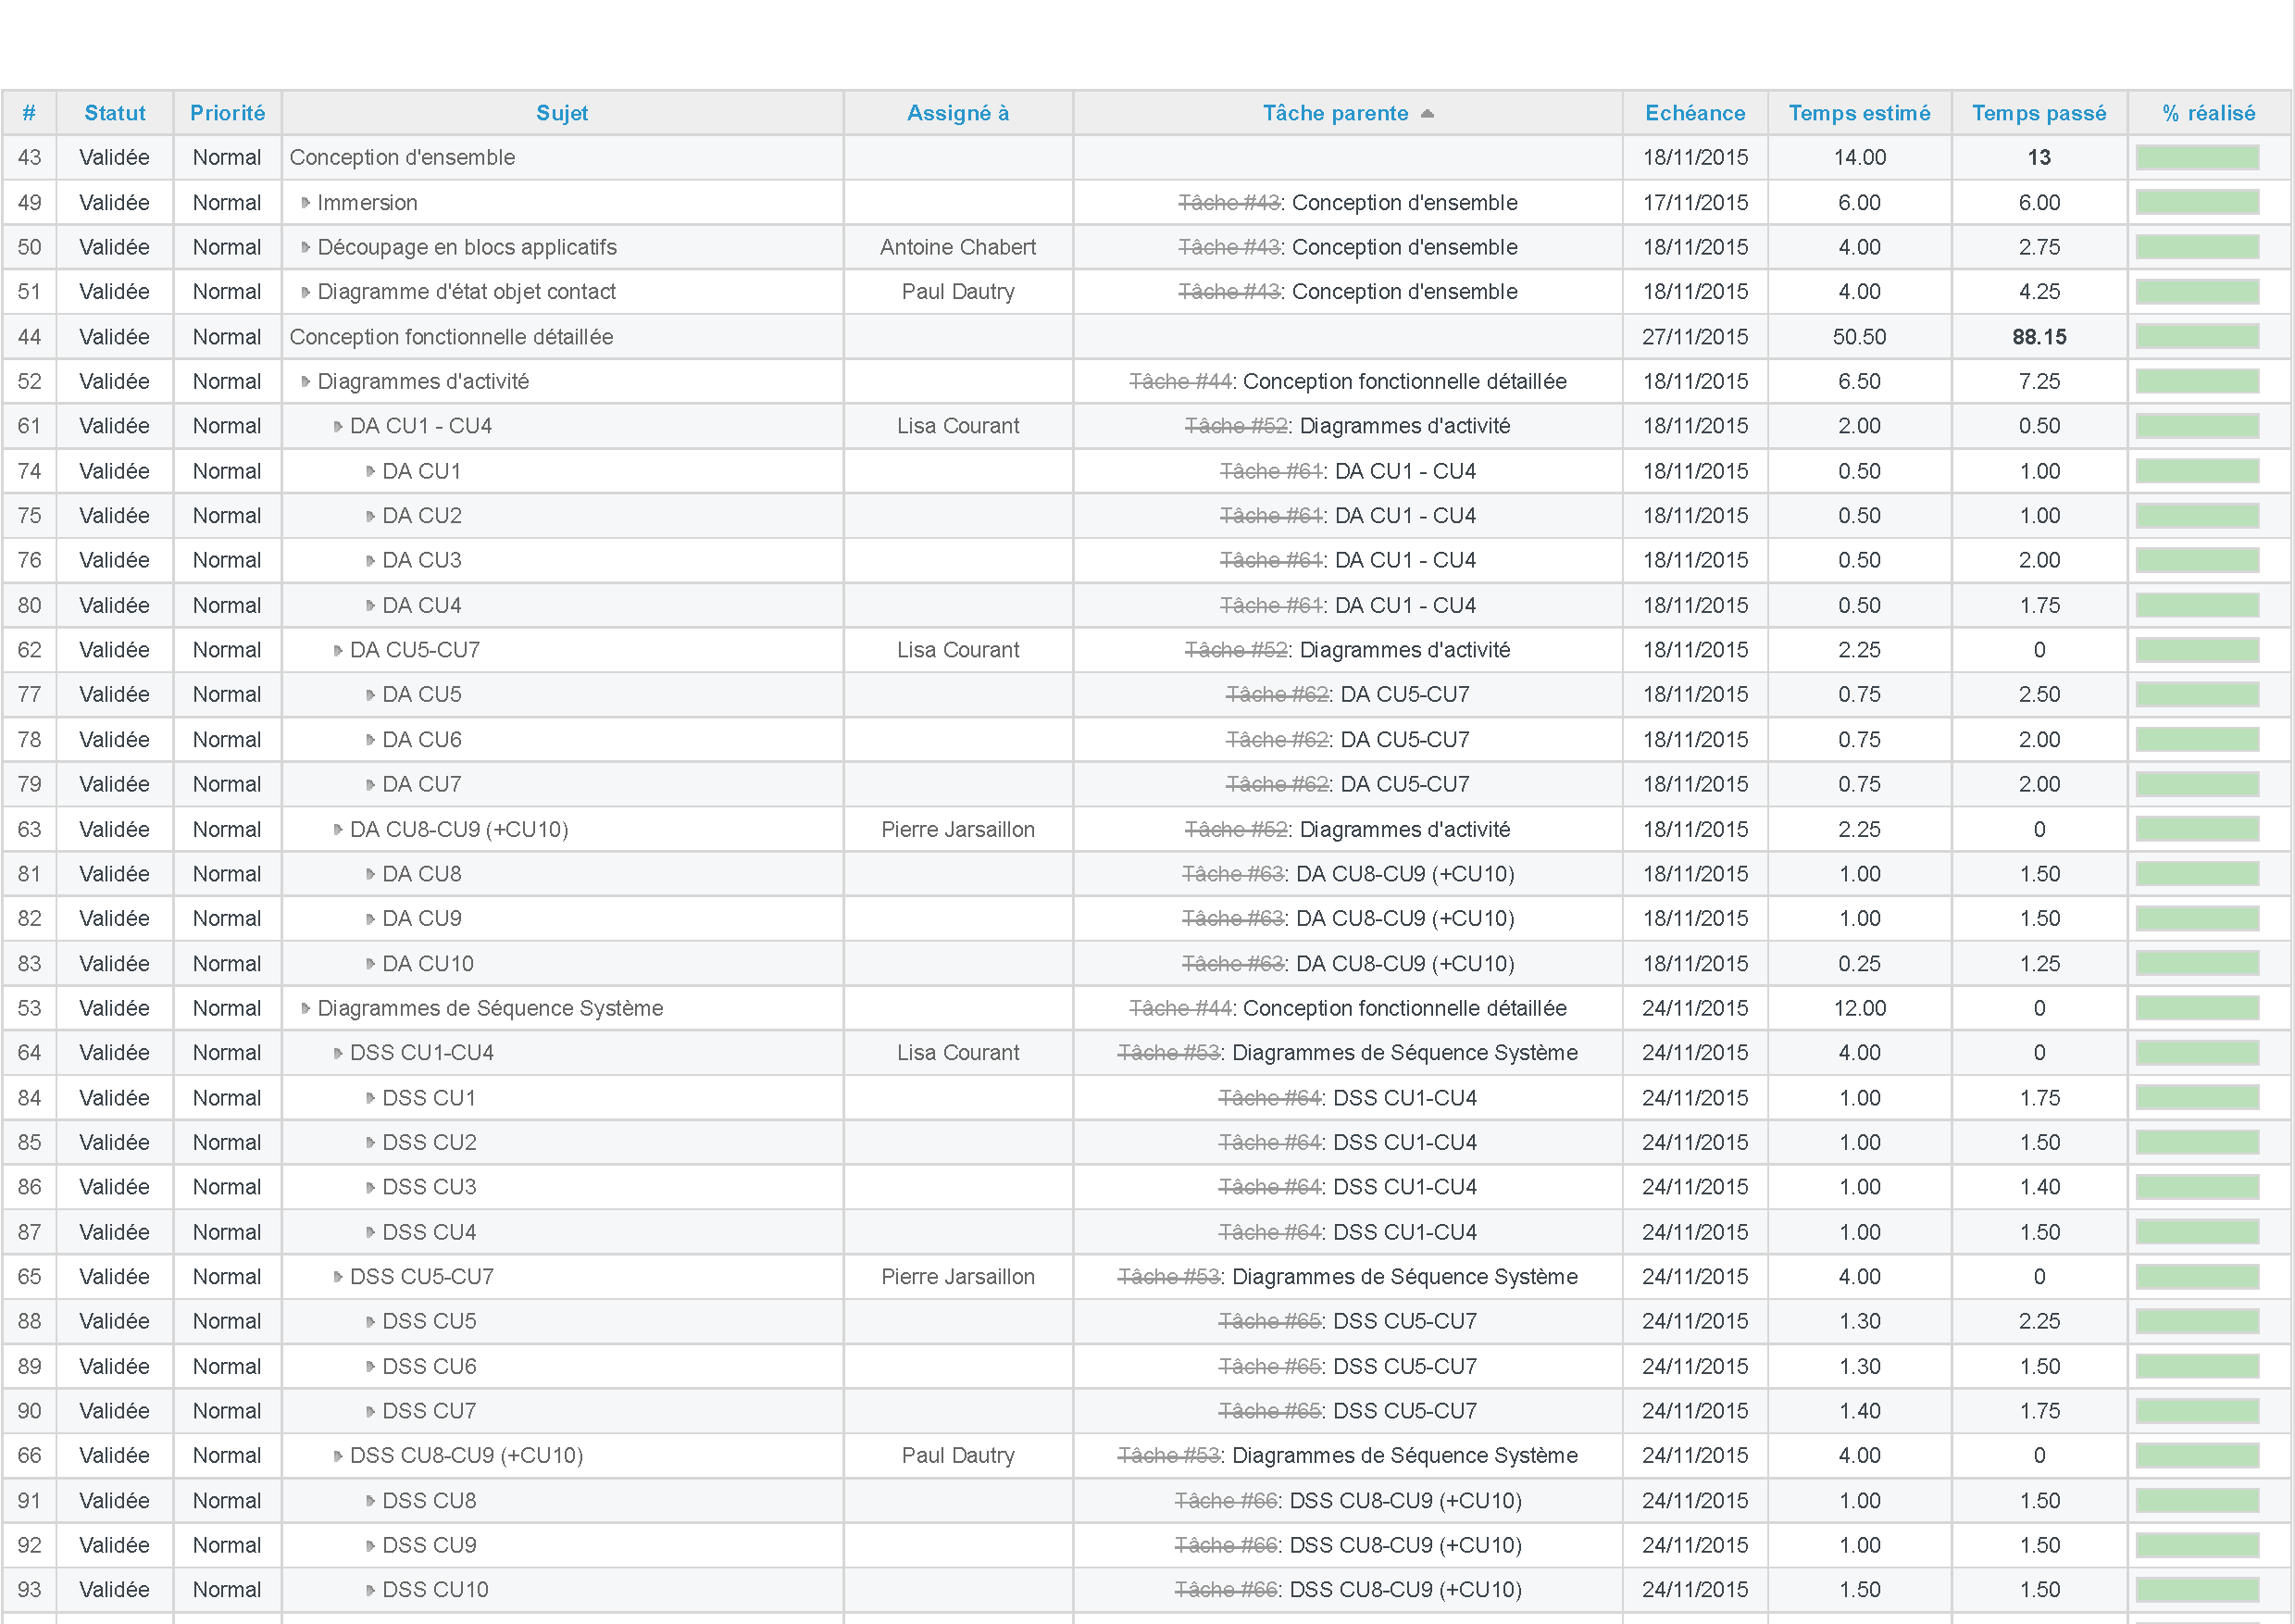
\includepdf[scale=0.8,angle=90,pages=-,pagecommand=\subsection*{IHM client}]{figures/avancement.pdf}

\begin{figure}[H]
\noindent\makebox[\textwidth]{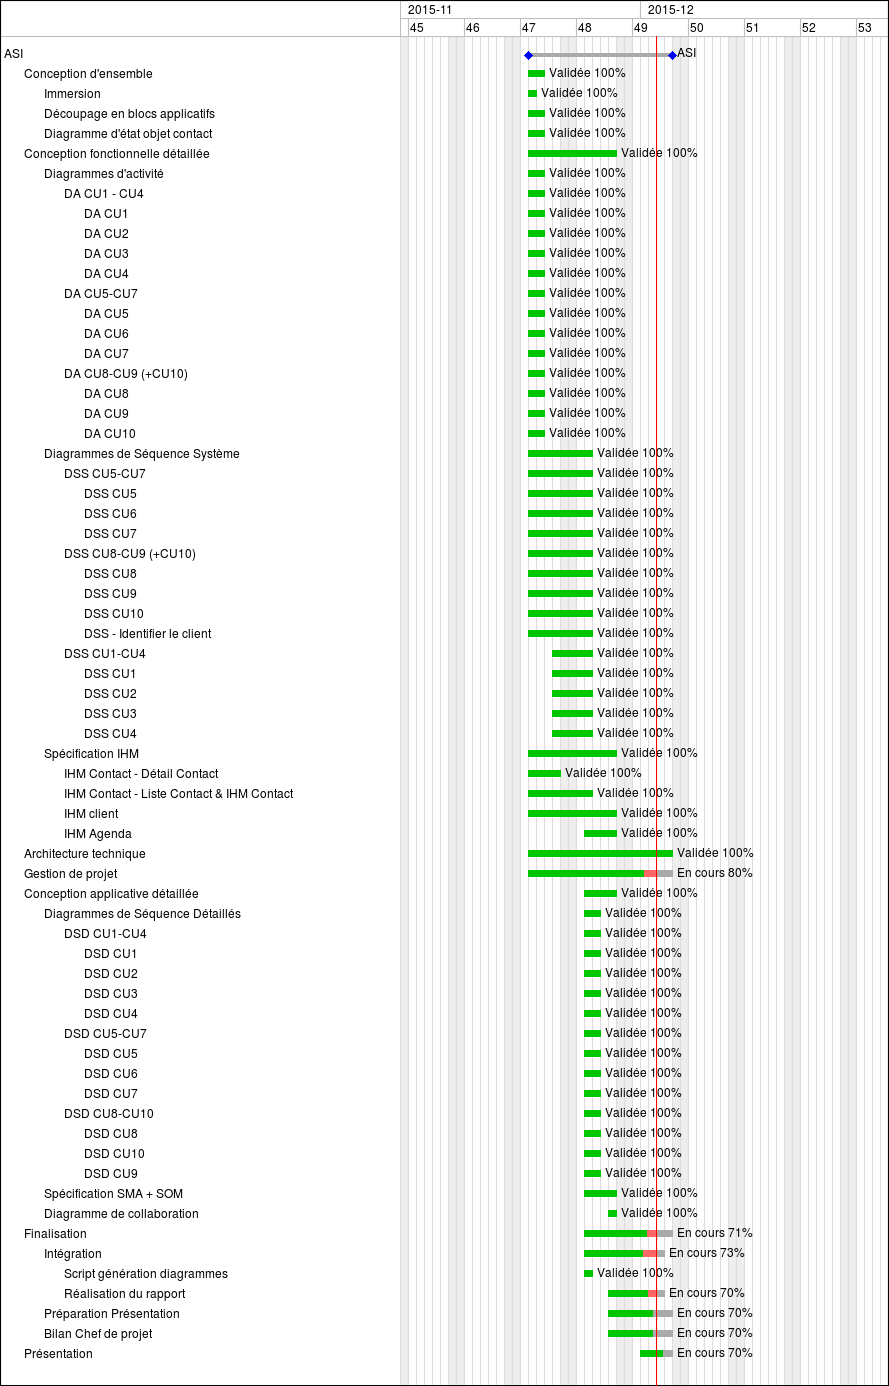
\includegraphics[width=16.5cm]{figures/asi-gantt.png}}
\caption{Gant du projet}
\end{figure}

\subsubsection*{Conception d'ensemble}
\subsubsection*{Conception fonctionnelle détaillée}
\subsubsection*{Conception applicative détaillé}

\section*{Conclusion}
\restoregeometry